\documentclass{beamer}

\usepackage{tikz-cd}
\usetikzlibrary{calc}

\definecolor{homcolor}{HTML}{1b9e77}

\begin{document}


%------------------------------------------------------------%


\begin{frame}[fragile]{simplicial homology}

\only<1>{
\begin{tikzpicture}
  % left component
  \coordinate (A) at (-1,-.5); \coordinate (B) at (.5,2); \coordinate (C) at (4,2); \coordinate (D) at (3,-1);
  %\draw (A) node {.}; \draw (B) node {.}; \draw (C) node {.}; \draw (D) node {.};
  \draw[smooth cycle,tension=1] plot coordinates{(A) (B) (C) (D)};
  % hole in left component
  \coordinate (P) at (2,1.5);
  \draw (P) arc(140:40:.5) (P) arc(-140:-20:.5) (P) arc(-140:-150:1);
  % right component
  \coordinate (W) at (5.5,-1); \coordinate (X) at (5,1); \coordinate (Y) at (7,2); \coordinate (Z) at (8.5,0);
  %\draw (W) node {.}; \draw (X) node {.}; \draw (Y) node {.}; \draw (Z) node {.};
  \draw[smooth cycle,tension=1] plot coordinates{(W) (X) (Y) (Z)};
  % cavity in right component
  \coordinate (Q) at (6.5,.5);
  \draw[dotted] (Q) circle (.4);
  % 2-simplex
  \coordinate (I) at (0,0); \coordinate (J) at (2,-.5); \coordinate (K) at (1.5,.75); \coordinate (L) at (.75,-.75);
  \coordinate (M) at (3.5,0); \coordinate (N) at (1.25,1.5); \coordinate (O) at (5.5,.667);
\end{tikzpicture}

\centering
\phantom{\(n\)-dimensional homology}
}
\only<2>{
\begin{tikzpicture}
  % left component
  \coordinate (A) at (-1,-.5); \coordinate (B) at (.5,2); \coordinate (C) at (4,2); \coordinate (D) at (3,-1);
  %\draw (A) node {.}; \draw (B) node {.}; \draw (C) node {.}; \draw (D) node {.};
  \draw[smooth cycle,tension=1] plot coordinates{(A) (B) (C) (D)};
  % hole in left component
  \coordinate (P) at (2,1.5);
  \draw (P) arc(140:40:.5) (P) arc(-140:-20:.5) (P) arc(-140:-150:1);
  % right component
  \coordinate (W) at (5.5,-1); \coordinate (X) at (5,1); \coordinate (Y) at (7,2); \coordinate (Z) at (8.5,0);
  %\draw (W) node {.}; \draw (X) node {.}; \draw (Y) node {.}; \draw (Z) node {.};
  \draw[smooth cycle,tension=1] plot coordinates{(W) (X) (Y) (Z)};
  % cavity in right component
  \coordinate (Q) at (6.5,.5);
  \draw[dotted] (Q) circle (.4);
  % 2-simplex
  \coordinate (I) at (0,0); \coordinate (J) at (2,-.5); \coordinate (K) at (1.5,.75); \coordinate (L) at (.75,-.75);
  \coordinate (M) at (3.5,0); \coordinate (N) at (1.25,1.5); \coordinate (O) at (5.5,.667);
  % 0-homology
  \filldraw [homcolor] (I) circle (2pt) (J) circle (2pt);
  \filldraw [homcolor] (3.5,0) circle (2pt) (5.5,-.5) circle (2pt);
  \draw [line width=1pt, homcolor] (I) -- (J);
  \draw [line width=1pt, dashed, homcolor] ($ (I) + (M) $) -- ($ (J) + (M) $);
\end{tikzpicture}

\centering
\(0\)-dimensional homology: {\bfseries gulfs}
}
\only<3>{
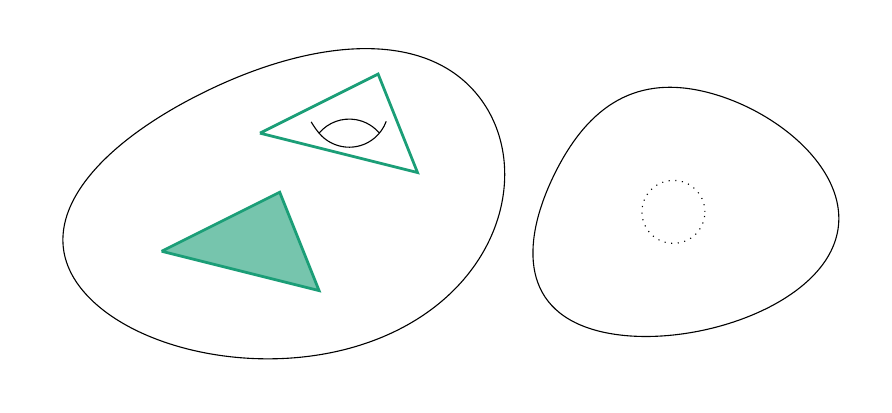
\begin{tikzpicture}
  % left component
  \coordinate (A) at (-1,-.5); \coordinate (B) at (.5,2); \coordinate (C) at (4,2); \coordinate (D) at (3,-1);
  %\draw (A) node {.}; \draw (B) node {.}; \draw (C) node {.}; \draw (D) node {.};
  \draw[smooth cycle,tension=1] plot coordinates{(A) (B) (C) (D)};
  % hole in left component
  \coordinate (P) at (2,1.5);
  \draw (P) arc(140:40:.5) (P) arc(-140:-20:.5) (P) arc(-140:-150:1);
  % right component
  \coordinate (W) at (5.5,-1); \coordinate (X) at (5,1); \coordinate (Y) at (7,2); \coordinate (Z) at (8.5,0);
  %\draw (W) node {.}; \draw (X) node {.}; \draw (Y) node {.}; \draw (Z) node {.};
  \draw[smooth cycle,tension=1] plot coordinates{(W) (X) (Y) (Z)};
  % cavity in right component
  \coordinate (Q) at (6.5,.5);
  \draw[dotted] (Q) circle (.4);
  % 2-simplex
  \coordinate (I) at (0,0); \coordinate (J) at (2,-.5); \coordinate (K) at (1.5,.75); \coordinate (L) at (.75,-.75);
  \coordinate (M) at (3.5,0); \coordinate (N) at (1.25,1.5); \coordinate (O) at (5.5,.667);
  % 1-homology
  \fill[fill=homcolor!60] (I) -- (J) -- (K) -- (I);
  \draw [line width=1pt, homcolor] (I) -- (J) -- (K) -- (I);
  \draw [line width=1pt, homcolor] ($ (I) + (N) $) -- ($ (J) + (N) $) -- ($ (K) + (N) $) -- ($ (I) + (N) $);
\end{tikzpicture}

\centering
\(1\)-dimensional homology: {\bfseries holes}
}
\only<4>{
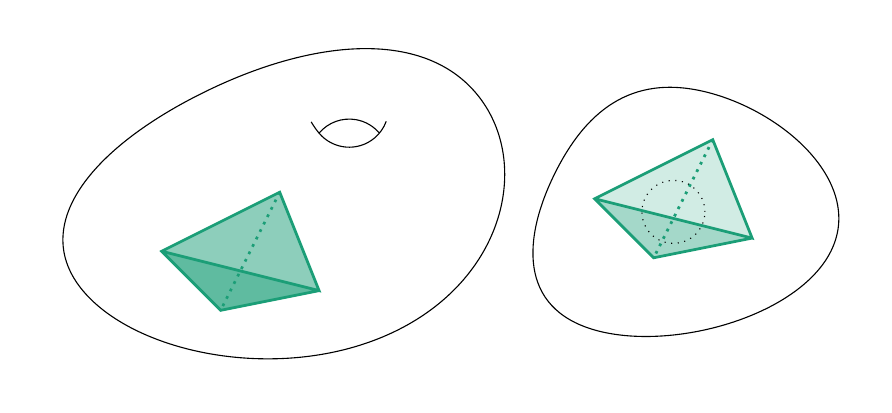
\begin{tikzpicture}
  % left component
  \coordinate (A) at (-1,-.5); \coordinate (B) at (.5,2); \coordinate (C) at (4,2); \coordinate (D) at (3,-1);
  %\draw (A) node {.}; \draw (B) node {.}; \draw (C) node {.}; \draw (D) node {.};
  \draw[smooth cycle,tension=1] plot coordinates{(A) (B) (C) (D)};
  % hole in left component
  \coordinate (P) at (2,1.5);
  \draw (P) arc(140:40:.5) (P) arc(-140:-20:.5) (P) arc(-140:-150:1);
  % right component
  \coordinate (W) at (5.5,-1); \coordinate (X) at (5,1); \coordinate (Y) at (7,2); \coordinate (Z) at (8.5,0);
  %\draw (W) node {.}; \draw (X) node {.}; \draw (Y) node {.}; \draw (Z) node {.};
  \draw[smooth cycle,tension=1] plot coordinates{(W) (X) (Y) (Z)};
  % cavity in right component
  \coordinate (Q) at (6.5,.5);
  \draw[dotted] (Q) circle (.4);
  % 2-simplex
  \coordinate (I) at (0,0); \coordinate (J) at (2,-.5); \coordinate (K) at (1.5,.75); \coordinate (L) at (.75,-.75);
  \coordinate (M) at (3.5,0); \coordinate (N) at (1.25,1.5); \coordinate (O) at (5.5,.667);
  % 2-homology
  \fill[fill=homcolor!50] (I) -- (J) -- (K); \fill[fill=homcolor!70] (I) -- (J) -- (L);
  \draw [line width=1pt, homcolor] (I) -- (J) -- (K) -- (I) -- (L) -- (J);
  \draw [line width=1pt, dotted, homcolor] (K) -- (L);
  \fill[fill=homcolor!20] ($ (I) + (O) $) -- ($ (J) + (O) $) -- ($ (K) + (O) $);
  \fill[fill=homcolor!40] ($ (I) + (O) $) -- ($ (J) + (O) $) -- ($ (L) + (O) $);
  \draw[dotted] (Q) circle (.4);
  \draw [line width=1pt, homcolor] ($ (I) + (O) $) -- ($ (J) + (O) $) -- ($ (K) + (O) $) -- ($ (I) + (O) $) -- ($ (L) + (O) $) -- ($ (J) + (O) $);
  \draw [line width=1pt, dotted, homcolor] ($ (K) + (O) $) -- ($ (L) + (O) $);
\end{tikzpicture}

\centering
\(2\)-dimensional homology: {\bfseries cavities}
}

\end{frame}


\end{document}
